\section{Daten-/Domänenmodell}
\subsection{Gegenstandwelt des Systems/Datenmodell}
\begin{figure}[h!]
    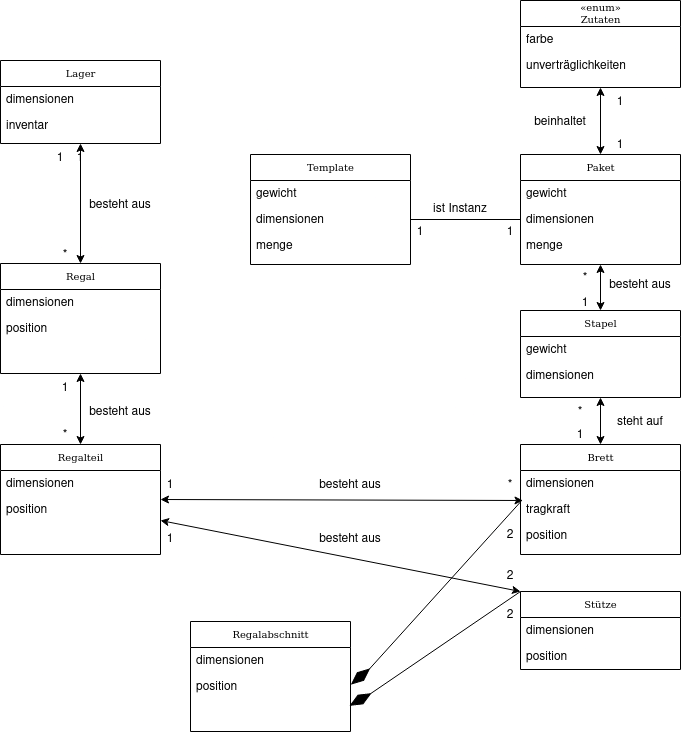
\includegraphics[width=\linewidth]{images/Domaenendiagramm.png}
    \captionbelow{Domänendiagramm}
    \label{fig:Domaenendiagramm}
\end{figure}
% Koordinaten von Stützen und Bretter relativ zu Lager/Regal?
% Bretter kennen ihre Pakete
% Pakete kennen ihre "Nachbarn"
% Stützen kennen ihre Bretter
% Bretter kennen ihre Stützen
% Wie bilden Regalabschnitte
% Wie positionieren wir ein Regal
\begin{figure}[H]
    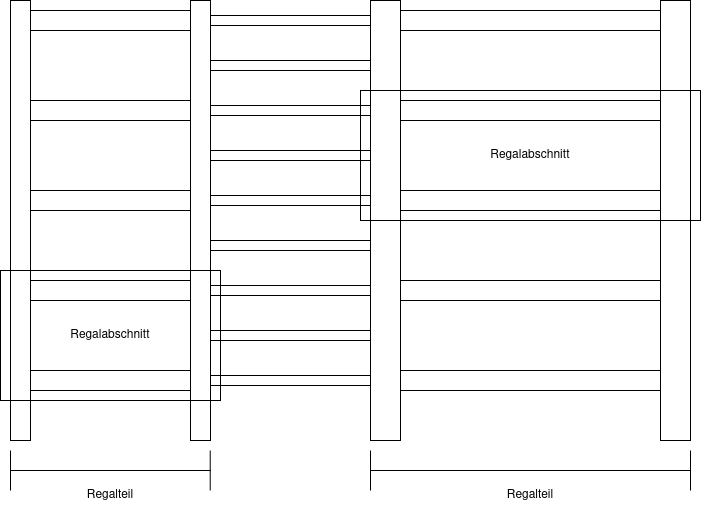
\includegraphics[width=\linewidth]{images/Regalmodell.png}
    \captionbelow{Regalmodell}
    \label{fig:Regalmodell}
\end{figure}
\subsection{Datentypenverzeichnis}
\textbf{Datentyp:} Dimensionen\\
\textbf{Beschreibung:} Beschreibt die Ausmaße einer Komponente (Höhe, Breite, Tiefe)\\
\textbf{Eigenschaften:}
\begin{itemize}
    \setlength\itemsep{0em}
    \item Höhe (Ganzzahl) in cm
    \item Breite (Ganzzahl) in cm
    \item Tiefe (Ganzzahl) in cm
\end{itemize}
\bigskip
\textbf{Datentyp:} Position\\
\textbf{Beschreibung:} Beschreibt eine zweidimensionale Positon im Raum\\
\textbf{Eigenschaften:}
\begin{itemize}
    \setlength\itemsep{0em}
    \item X (Ganzzahl) in cm
    \item Y (Ganzzahl) in cm
\end{itemize}
\textbf{Datentyp:} Lager\\
\textbf{Beschreibung:} Modellierung eines bestimmten Raums\\
\textbf{Eigenschaften:}
\begin{itemize}
    \setlength\itemsep{0em}
    \item dimensionen (Dimensionen)
    \item inventar (Liste von Paketen)
\end{itemize}
\bigskip
\textbf{Datentyp:} Regal\\
\textbf{Beschreibung:} Eine Komposition aus Stützen und Brettern\\
\textbf{Eigenschaften:}
\begin{itemize}
    \setlength\itemsep{0em}
    \item position (Position)
    \item regalteile (Liste von Regalteilen)
\end{itemize}
\bigskip
\textbf{Datentyp:} Regalteil\\
\textbf{Beschreibung:} Ein durch zwei Stützen begrenzter Teil eines Regals\\
\textbf{Eigenschaften:}
\begin{itemize}
    \setlength\itemsep{0em}
    \item position (Position)
    \item bretter (Liste von Brettern)
    \item stützen (2 Stützen)
\end{itemize}
\bigskip
\textbf{Datentyp:} Regalabschnitt\\
\textbf{Beschreibung:} Ein Bereich des Regals, der durch zwei Stützen und zwei Bretter abgetrennt wird\\
\textbf{Eigenschaften:}
\begin{itemize}
    \setlength\itemsep{0em}
    \item position (Position)
    \item bretter (2 Brettern)
    \item stützen (2 Stützen)
\end{itemize}
\bigskip
\textbf{Datentyp:} Brett\\
\textbf{Beschreibung:} Ein horizontales Brett in einem Regal\\
\textbf{Eigenschaften:}
\begin{itemize}
    \setlength\itemsep{0em}
    \item Y (Ganzzahl) in cm, relativ zu Regal
    \item dimensionen (Dimensionen)
    \item tragkraft (Ganzzahl) in kg
\end{itemize}
\bigskip
\textbf{Datentyp:} Stütze\\
\textbf{Beschreibung:} Ein vertikales Brett in einem Regal\\
\textbf{Eigenschaften:}
\begin{itemize}
    \setlength\itemsep{0em}
    \item X (Ganzzahl) in cm, relativ zu Regal
    \item dimensionen (Dimensionen)
\end{itemize}
\bigskip
\textbf{Datentyp:} Paket\\
\textbf{Beschreibung:} Eine bestimmte Packung einer Zutat im Regal\\
\textbf{Eigenschaften:}
\begin{itemize}
    \setlength\itemsep{0em}
    \item gewicht (Ganzzahl) in kg
    \item dimensonen (Dimensionen)
    \item menge (Ganzzahl) in kg
    \item zutat (Zutat)
\end{itemize}
\bigskip
\textbf{Datentyp:} Stapel\\
\textbf{Beschreibung:} Ein Stapel, der auf einem Brett steht\\
\textbf{Eigenschaften:}
\begin{itemize}
    \setlength\itemsep{0em}
    \item pakete (Liste von Paketen)
    \item dimensonen (Dimensionen)
    \item gewicht (Ganzzahl) in kg
\end{itemize}
\bigskip
\textbf{Datentyp:} Template\\
\textbf{Beschreibung:} Eine Vorlage für eine Packung\\
\textbf{Eigenschaften:}
\begin{itemize}
    \setlength\itemsep{0em}
    \item gewicht (Ganzzahl) in kg
    \item dimensionen (Dimensionen)
    \item menge (Ganzzahl) in kg
    \item zutat (Zutat)
\end{itemize}
\bigskip
\textbf{Datentyp:} Zutat\\
\textbf{Beschreibung:} Eine Zutat der Pizzeria\\
\textbf{Eigenschaften:}
\begin{itemize}
    \setlength\itemsep{0em}
    \item farbe (Color)
    \item unverträglichkeiten (Liste von Zutaten)
\end{itemize}